\documentclass[10pt,a4paper,twoside]{article}

\usepackage[T1]{fontenc}
\usepackage[latin1,utf8]{inputenc}

\usepackage{lmodern}

\usepackage[pdftex]{graphicx} 

\usepackage[tracking=true]{microtype}
               
                               
\usepackage{amsmath,amssymb,amsthm}
\usepackage{xfrac}
\usepackage{mathrsfs}
\usepackage{mathtools}
\usepackage{grffile}  

\usepackage{bbm} %for use of identity-matrix
\usepackage{dsfont}

\usepackage[]{subfigure}
\usepackage{wrapfig}
\usepackage{multicol}

\usepackage{verbatim}
\usepackage{setspace}

\usepackage{color}
\usepackage[]{hyperref}

\usepackage{accents}
\usepackage{textcomp}
\usepackage{multirow}
\usepackage{booktabs}
\usepackage{float}

\usepackage[numberedbib]{apacite}
\bibliographystyle{apacite}
\usepackage[flushleft]{threeparttable}
\usepackage{tabulary}
\usepackage{indentfirst}


\usepackage{geometry}
\geometry{a4paper,left=30mm,right=25mm, top=20mm, bottom=25mm}

\usepackage{fancyhdr}
\pagestyle{fancy}
\fancyhf{}
\rhead{André Crescenzo}
\lhead{Computer-aided Design of Bio-inspired Nanoporous Silica Materials}
\lfoot{\today}
\rfoot{\thepage}

\usepackage{abstract}
\usepackage{authblk}

\title{A Coarse-grain model for Bolaamphiphiles in presence  of Silica}
\author[1,2]{André Crescenzo\thanks{ Corresponding author.\\ Email: \ \texttt{andre.crescenzo.2014@uni.strath.ac.uk}}}
\author[1]{Alessia Centi\thanks{ Email: \ \texttt{alessia.centi@strath.ac.uk}}}
\author[1]{Miguel Jorge\thanks{Email: \ \texttt{miguel.jorge@strath.ac.uk}}}
\affil[1]{Department of Chemical and Process Engineering, University of Strathclyde}
\affil[2]{Departamento de Engenharia Química da Escola Politécnica, Universidade de São Paulo}
\renewcommand\Authands{ and }
\date{\today \\
\begin{abstract}
\textbf{Aim:} Finish my job!\\
\textbf{Conclusion:}Repeating the results is not drawing a conclusion.
\begin{tabular}
& \textbf{Keywords}: Latex$\cdot$ Bibtex  $\cdot$ Scientific Paper $\cdot$ More Scientific Papers $\cdot$ More Scientific Papers  $\cdot$ More Scientific Papers $\cdot$ More Scientific Papers $\cdot$ More Scientific Papers $\cdot$ More Scientific Papers 
\end{tabular}
\end{abstract}}

\pagenumbering{roman}

\begin{document}
%\doublespace
\begin{titlepage}

\newcommand{\HRule}{\rule{\linewidth}{0.5mm}} 

\center 
 
\begin{figure*}[ht!]
	
\includegraphics[width=1 \textwidth]{./images/StrathLogo}
\end{figure*}


\textsc{\LARGE University of Strathclyde}\\[1.5cm] 
\textsc{\Large Department of Chemical \& Process Engineering}\\[0.5cm] 
\textsc{\large M.Eng Chemical \& Process Engineering 18530}\\[0.5cm] 


\HRule \\[0.4cm]
{ \huge \bfseries Computer-aided Design of Bio-inspired Nanoporous Silica Materials}\\[0.4cm] % Title of your document
\HRule \\[1.5cm]
 

\begin{minipage}{0.4\textwidth}
\begin{flushleft} \large
\emph{Author:}\\
André \textsc{Crescenzo} 
\end{flushleft}
\end{minipage}
~
\begin{minipage}{0.4\textwidth}
\begin{flushright} \large
\emph{Supervisor:} \\
Miguel \textsc{Jorge} 
\end{flushright}
\end{minipage}\\[4cm]

{\large \today}\\[3cm] % Date, change the \today to a set date if you want to be precise


\vfill 

\end{titlepage}
\addtocontents{toc}{~\hfill\textbf{Page}\par}
\section{Summary}
\setcounter{page}{1}

\vfill
\newpage

\setcounter{tocdepth}{3}
\tableofcontents



\vfill
\newpage

\section{Acknowledgements}

\vfill
\newpage

\pagenumbering{arabic}
\section{Introduction}
%%%%%%%%%%%%%%%%%%%%%%%%%%%%%%%%%%%%%%%%%%%%%%%%%%%%%%%%%%%%%%%%%%%%%%%%%%%%%%%%%%%%%%%%%%%%%%%%%%%%%%
%A good introduction is a clear statement of the problem or project and the reasons for studying it. 
%This information should be contained in the first few sentences.										
%Give a concise and appropriate background discussion of the problem									
%and the significance, scope, and limits of the work. Outline what has been done						
%before by citing truly pertinent literature, but do not include a general survey of					
%semirelevant literature. State how your work differs from or is related to work						
%previously published. Demonstrate the continuity from the previous work to yours.					
%The introduction can be one or two paragraphs long. Often, the heading								
%“Introduction” is not used because it is superfluous; opening paragraphs are usually introductory	
%%%%%%%%%%%%%%%%%%%%%%%%%%%%%%%%%%%%%%%%%%%%%%%%%%%%%%%%%%%%%%%%%%%%%%%%%%%%%%%%%%%%%%%%%%%%%%%%%%%%%%
 %clear statement of the problem + reasons for studying it\\
 
Molecular Dynamics (MD) and Monte Carlo (MC) have been powerful tools to simulate molecular interactions of surfactants in solvent systems, allowing a deeper understanding of self-assembly process of this sort of material \cite{someone}. Therefore, these structural conformations are specially useful to design bio-inspired silica materials \cite{bioinsp} since with the addition of silica they remain behaving as scaffolds to mesoporous or nanoporous structures that are maintained even after surfactant removal, silica oligomer polymerization and calcination \cite{silica1}.
A vast range of silica materials are examples of this phenomena, such as MCM-41 as reported by \citeA{mcm}, HR \cite{hrib}, MSU-V \cite{msuv} and many others, in which the self-assembly structure depend on the type of surfactant and concentration of the substances involved. Moreover, most of the experimental methods used to obtain data are based on observation and interpretation of final silica structure by using X-ray diffraction (XRD) and transmission electron microscopy (TEM), thus initial self-assembled conformations are predicted as a reflex of the final results and little is known about the mechanistic of this process. However, by using MD simulations it is possible to observe and analyse these initial steps of self-assembly and further predict, with more accuracy, properties and framework provided by surfactant \cite{lipid} to generate silica structures.

%  background discussion\\
%  what has been done by others(cite works)\\
A major concern is that even though MD uses sophisticated software prepared to simulate enormous systems with thousands of atoms, using all capacities of hardware available, such as high-speed multi-core processors in conjunction with GPUs designed specifically to process data from arrays \cite{gromacs}, they hardly can achieve long time horizons and are commonly limited to a few $\mu s$ depending on the size of the system. For this reason, several techniques have been develop to optimize the performance of the simulations such as coarse-grain models \cite{someone}. Briefly, the idea behind using this technique is to fit parameters of heavy atoms groups with similar properties in a bigger "bead", which includes atomic masses and electrostatic charges lumped in approximated values. For example, by merging carbon heavy atoms, that means carbon atom and its hydrogen atoms, at a lipid tail in groups of three or four since they have similar hydrophobic properties. 

%  how mine differs from the others\\
%  how it relates to the others\\
In order to provide topologies to GROMACS simulations several force-fields, for exemple MARTINI \cite{martini}, use Lennard-Jones potentials fitted to a range of pre-defined bead types to describe coarse-grain models. Furthermore, not only intramolecular beads are possible, but also intermolecular beads can be specified, such as multiple solvent molecules merged in a single bead or ions surround by water molecules. Previous works conducted by \cite{mjsilica} with this method recreated a model of surfactant in presence of silica with explicit water that was successful in describing rod-like self-assembly structures detected on MCM-41 materials, demonstrating the capacities of up-scaling this type of systems. Nevertheless, solvent presence demands most of the computational resources, hence  implicit solvent scheme has been focus of many studies \cite{gromacs}.

Different concepts has been applied to develop a suitable model for implicit solvents, studies conducted by \citeA{drymartini} developed the Dry MARTITNI force-field by modifying parameters of its predecessor, in such manner that solvent interactions became incorporated in these values and then solvent beads are no longer necessary. Another method, described by \cite{magic} is able to recreate a implicit solvent system from interaction potentials generated from a bottom-up approach, that means by using an all-atoms simulation to generate parameters for the coarse-grain model. It is supposed  that thermodynamic changes on the system, originated from solvent interaction with amphiphilic molecules, are incorporated on the approximated potentials. Therefore, changes in parameters as concentration may not affect coarse-grained model performance on recreating self-assembly structures \cite{dmpc}.

%  significance of the work\\
%  scope of the work\\
%  limts of the work\\
The work presented on following experiments are an attempt to create a cross-link method to upscale silica crystal-liquid phase interactions \cite{silica1} from the atomistic model to a mesoscale model with the advent of this later coarse-grain technique. The methodology applied to reach the desired model is based on the MagiC software package \cite{magic} that in conjunction MD simulation software, in this case GROMACS \cite{gromacs}, will provide a suitable approximation to self-assembly of amphiphilic molecules in presence of silica. Further explanations of the process are described on Experimental Methods section. For the scope of this project, a bolaamphiphilic molecule 1,12-diaminododecane (DMDD) has been chosen as surfactant because that as seen in previous research by \citeA{msuv} it self-assembly in multilamelar vesicles that in presence of a silica precursor is capable of generating a mesoporous structure with remarkable properties. In order to validate this structure formation and further framework formation for silica oligomers, a coarse-grain approximation is suitable option since amphiphilic molecules interaction with solvents can be described efficiently with tabulated Lennard-Jones potentials interactions. As a final objective at the end of this project, a implicit water coarse-grain model for DMDD will be generated and properly validated based on MD simulations and thermodynamic properties,in order to provide a good approximation to interactions with silica oligomers in a mesoscale model. 
%  continuity?(maybe silica interactions...)\\
\section{Experimental Methods}
\subsection{Theoretical Basis}
This work is based on two molecular simulation techniques the former, called Molecular Dynamics, accounts for integration of Newton forces in order to describe positions and velocities of particles in the system. The latter, called Monte Carlo method, is a powerful statistical tool based on stochastic inputs to measure properties of many systems, in this case thermodynamic equilibrium of molecular systems. Following sections will describe the mechanistic behind each technique and further explain how they are used in simulation software.
\subsubsection*{Molecular Dynamics simulation}

Molecular Dynamics is a simulation method that originates from dynamic nature of atomic interactions. Generally, a system of atoms can be treated as a multi-particle system ruled by Newton's Law \cite{umd}. Considering a system with $\mathcal{N}$ atoms for each $i$th particle of the system the follow differential equation:
\begin{equation}
m_i\dfrac{\,d^2\vec{r}_i(t)}{\,dt^2} = \vec{F}_i(t)
\label{eqn:newton}
\end{equation}

Where $\vec{r} = (x,y,z)$ is the position vector and $F = (F_x, F_y, F_z)$ are the force components. Therefore, for this $\mathcal{N}$ particle system, it is necessary to solve $3\mathcal{N}$ differential equations in order to fully describe it analytically at any $t$. Since any molecular system involves an enormous number of molecules, solving these equations analytically is impracticable and simulation methods are necessary.The derivatives terms need to be numerically calculated and as soon as simulation efficiency is a major concern, a suitable approximation to the second derivative of position is the Taylor's expansion, taking the x coordinate as an example, for a given $\Delta t$ is:
\begin{equation}
x(t+\Delta t) = x(t) + \Delta t \dfrac{\,dx(t)}{\,dt} + \dfrac{1}{2!}{\Delta t}^2 \dfrac{\,d^2x(t)}{\,dt^2} + \dfrac{1}{3!}{\Delta t}^3 \dfrac{\,d^3x(t)}{\,dt^3} +  \mathcal{O}(\Delta t^4)
\label{eqn:taylor1}
\end{equation}
\begin{equation}
x(t-\Delta t) = x(t) - \Delta t \dfrac{\,dx(t)}{\,dt} + \dfrac{1}{2!}{\Delta t}^2 \dfrac{\,d^2x(t)}{\,dt^2} - \dfrac{1}{3!}{\Delta t}^3 \dfrac{\,d^3x(t)}{\,dt^3} +  \mathcal{O}(\Delta t^4)
\label{eqn:taylor2}
\end{equation}
\begin{equation}
\dfrac{\,d^2x(t)}{\,dt^2} = \dfrac{x(t+\Delta t) - 2 x(t) + x(t-\Delta t)}{{\Delta t}^2} +  \mathcal{O}(\Delta t^2)
\label{eqn:dx2}
\end{equation}

Hence, by neglecting the error of order $\mathcal{O}(\Delta t^2)$, it is possible to use equations Eqn.(\ref{eqn:newton}) and Eqn.(\ref{eqn:dx2}) to derive the called "Verlet method" where position and velocity vectors for each $i$th atom on next step ($t+\Delta t$) are calculated using previous and current step:
\begin{equation}
\vec{r}_i(t+\Delta t) = 2 \vec{r}_i(t) - \vec{r}_i(t-\Delta t) + \dfrac{{\Delta t}^2}{m_i}\vec{F}_i(t)
\label{eqn:verletr}
\end{equation}
\begin{equation}
\vec{v}_i(t) =  \dfrac{\vec{r}_i(t+\Delta t) - \vec{r}_i(t-\Delta t)}{2{\Delta t}}
\label{eqn:verletv}
\end{equation}

In order to improve accuracy on Verlet method, another approach can be made by accounting a new force term in the velocity. This term is calculated from the updated position vector, and this improved velocity term is used to calculate the new position in the next step, creating a preciser step cycle with more stability\cite{satoh}. This set of equations are called "Velocity Verlet method" and they are described as:
\begin{equation}
\vec{r}_i(t+\Delta t) = \vec{r}_i(t) + \vec{v}_i(t)\Delta t + \dfrac{\vec{F}_i(t)}{2m_i}{\Delta t}^2
\label{eqn:vverletr}
\end{equation}
\begin{equation}
\vec{v}_i(t+\Delta t) = \vec{v}_i(t) + \dfrac{\vec{F}_i(t+\Delta t)+\vec{F}_i(t)}{2m_i}\Delta t
\label{eqn:vverletv}
\end{equation}

As a final variation for Verlet method one can derive the "Leap frog method", in which considers half-step when calculating the velocity term. Even though the use of this technique leads to a more stable and accurate behaviour when compared to Verlet method, it is noticeable that velocity and position are not in the same time steps, therefore it is not possible to calculate the total energy at a given $t$, just kinetic or potential energy separately \cite{umd}. By applying first-order derivatives with half-steps, one can obtain the following equations:
\begin{equation}
\vec{r}_i(t+\Delta t) = \vec{r}_i(t) + \vec{v}_i(t+\sfrac{\Delta t}{2})\Delta t
\label{eqn:leapfrogr}
\end{equation}
\begin{equation}
\vec{v}_i(t+\sfrac{\Delta t}{2}) = \vec{v}_i(t-\sfrac{\Delta t}{2}) + \dfrac{\vec{F}_i(t)}{m_i}\Delta t
\label{eqn:leapfrogv}
\end{equation}

The force term for each step is a key factor to define whether Molecular Dynamics are realistic or not. They are strictly related to the force-field adopted to describe molecular interactions, since they provide parameters to describe Lennard-Jones potentials in which forces can be calculated at any system configuration. Eventually, as seen in innovative methods such as the used on this project, the potential values can also be provided by tables generated specifically for each molecular interaction, explanations about this technique will be given on further sections. Molecular dynamics technique enable the use of thermostats and barostats to control dynamic behaviour of temperature and pressure of the system, recreating different types of thermodynamic ensemble. Hence, at equilibrated states, system properties can be obtained as a temporal average of instantaneous values and those averages can be compared to real experimental data in order to validate simulations.

\subsubsection*{Monte Carlo simulation}
Monte Carlo is  a simulation method based on statistical probability of existence of a system at thermodynamic equilibrium. This happens when free energy reaches a minimum by calculating the energy for each particle's microscopic state. Given a system of $ \mathcal{N}$ particles, temperature $T$ and volume $V$, thus it can be denoted as a canonical ensemble, it is possible to assume that  the free Helmholtz energy of the system is:
\begin{equation}
A = U - TS
\label{eqn:freeE}
\end{equation}

Where $S$ is the entropy and $U$ is the internal energy, meaning that not only a minimum in free energy can arise from a minimum in total energy, but also an increase in entropy of the system can contribute to this energy minimization. A system can be described by a group of coordinates, in this case to give a simplified idea assume a group of distance vectors $\lambda = (	\vec{r}_1,\vec{r}_2, \ldots, \vec{r}_\mathcal{N} )$ from system origin. For an arbitrary $\lambda$ the probability of a single particle of the system to statistically occupy that position is described by using a probability distribution function \cite{satoh}:
\begin{equation}
\rho(\lambda) = \dfrac{\exp{\left(-\dfrac{U(\lambda)}{kT}\right)}}{\displaystyle \int_V \dots   \int_V \exp{\left(-\dfrac{U(\lambda)}{kT}\right)}\,d\vec{r}_1 \,d\vec{r}_2 \ldots \,d\vec{r}_\mathcal{N} }
\label{eqn:rho}
\end{equation}

Whether the system configuration is generated with considerable number of microstates that satisfies this probability, the final configuration would have a real physical meaning. But, as soon as it is almost impossible to define an analytical solution to this equation if $\mathcal{N}$ is too large another method became necessary to use Monte Carlo simulations in molecular dynamics. The Metropolis method \cite{metropolis} allowed the use of Monte Carlo technique by introducing the following concept: given 2 different microstates, the probability to change from state 1 to 2 is defined by:

\begin{equation}
 P_{1\mapsto2} = \left\{
\begin{array}{c l}     
    1 & for \ \frac{\rho(\lambda_2)}{\rho(\lambda_1)}\geqslant1\\
    \dfrac{\rho(\lambda_2)}{\rho(\lambda_1)} & for \ \frac{\rho(\lambda_2)}{\rho(\lambda_1)}<1
\end{array}\right.
\label{eqn:metrop}
\end{equation}

 Therefore, the integral term in eq.(\ref{eqn:rho}) vanishes and it is clear to observe that when $U(\lambda_1) \geqslant U(\lambda_2)$ the system will certainly change to this new microstate since it has lower energy, however in the case of $U(\lambda_1) < U(\lambda_2)$ the system has a certain probability of changing to this new microstate indicating an increase of entropy in the system. So, by applying stochastic inputs for particle displacements and acceptance values for eq.(\ref{eqn:metrop}), with a large number of Monte Carlo steps the system will eventually reach a minimum in free energy.
  Moreover, when this system reaches equilibrium it is possible to calculate accurately microstate dependent properties via ensemble averages. That means with $n$ samples of Monte Carlo steps, the average of a $ \xi $ property can be obtained by:
 
 \begin{equation}
\left\langle \xi\right\rangle  = \displaystyle \sum_{i=1}^{n} \dfrac{\xi_i}{n}
\label{eqn:average}
\end{equation}

It is important to notice that Monte Carlo simulations do not consider dynamic properties of the system such as kinetic energy, and therefore only Molecular Dynamics can account such things\cite{satoh}. Finally, now that both molecular simulation methods had been properly introduced it is possible to proceed to an overview of both simulation software used on this project. Together they can unite the benefits of both simulation methods, in order to recreate a suitable coarse-grain model for Molecular Dynamics.

\subsubsection*{About GROMACS}

 GROMACS (\textbf{Gro}ningen \textbf{Ma}chine for \textbf{C}hemical \textbf{S}imulations) \cite{gromanual} is a Molecular Dynamics and energy minimization software created at the University of Groningen (the Netherlands), and currently has been developed and updated by Royal Institute of Technology and Uppsala University (Sweden). GROMACS is a widely used tool in the branch of computational chemistry because it is flexible and efficient. Its flexibly comes from the capacity of simulating multiscale molecular models, from atomistic to mesoscale depending on topology described by the user. The efficiency originates from the computational optimisation, by this meaning not only that GROMACS can achieve impressive simulation speed in large system using supercomputing or clusters, but also it can run small simulations in any ordinary computers with great performance.
 
 In order to interpret interatomic interactions, that means forces between each pair of atoms, GROMACS uses pre-defined parameters called Topologies in which the user can describe almost any molecule using force fields or tabled potentials. Data given in this description includes information regarding atoms' type, mass and charge. Furthermore, it includes detailed description of each angle and dihedral for the molecule. There are several Force-fields available for usage depending on the desired objective of the simulation, their role is to be a database that describes interactions potential, hence their applicability is suitable to almost any system from all-atoms to coarse-grain descriptions it is just necessary for the user to describe a realistic model.
 
  When dealing of simulations of complex systems, realism means more computational power expended trying to achieve it\cite{satoh}, therefore a major concern is how to achieve longer time horizons without loosing precision. A good example is the Lennard-Jones potential for Van der Waals forces, used by OPLS-AA Force-field \cite{opls}, which is the one chosen for all-atomic simulations in this project. This type of potential approximation for a given atom $i$ in relation to atom $j$ is defined simply by two parameters  $\epsilon$ and $\sigma$ as it can be seen in Eq.\ref{eqn:ljpot}:

\begin{equation}
\mathcal{U}_{LJ}(r_{ij}) = 4\epsilon_{ij}\left(\left( \dfrac{\sigma_{ij}}{r_{ij}}\right)^{12} - \left( \dfrac{\sigma_{ij}}{r_{ij}}\right)^6\right) 
\label{eqn:ljpot}
\end{equation}

 \begin{figure}[ht]
  \begin{center}
	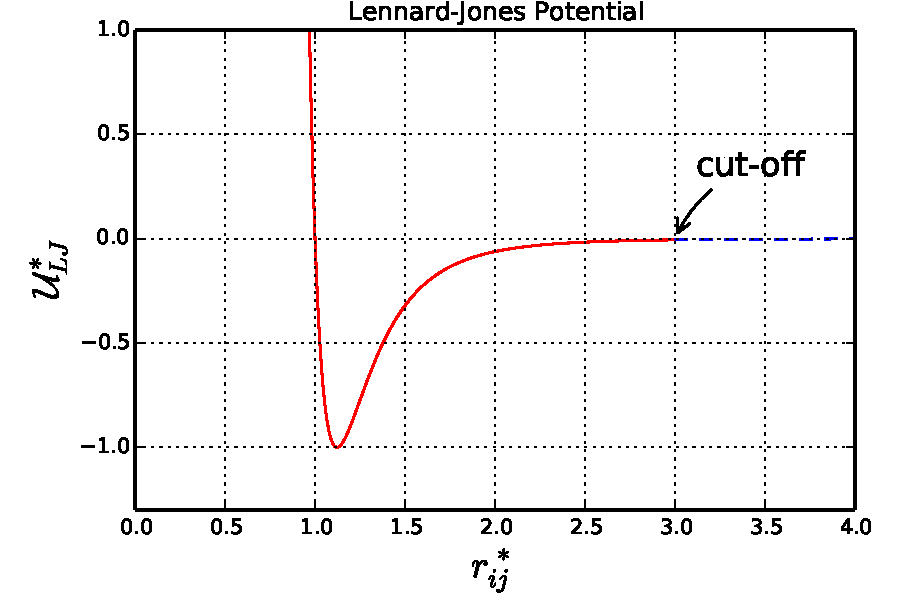
\includegraphics[width=0.6 \textwidth]{./graphs/lj}
	\caption{Example of Lennard-Jones Potential(with reduced units)}
	\label{gfx:ljg}
	\end{center}
	\end{figure}

Where the forces used in Molecular Dynamics equations come from derivative of this potential for each pair of particles:
\begin{equation}
\vec{F}_{ij} = \nabla\mathcal{U}_{LJ}(r_{ij}) = \left( \dfrac{\partial\mathcal{U}_{LJ}(r_{ij})}{\partial x}\hat{x} + \dfrac{\partial\mathcal{U}_{LJ}(r_{ij})}{\partial y}\hat{y}+\dfrac{\partial\mathcal{U}_{LJ}(r_{ij})}{\partial z}\hat{z}\right) 
\label{eqn:ljf}
\end{equation}

For every simulation time-step, GROMACS recalculates bonded potentials from Topology, and non-bonded potentials from the summation of Lennard-Jones and short-range Coulomb potentials. As shown in Fig.(\ref{gfx:ljg}) whether $r_{ij} \rightarrow \infty$ $\Rightarrow$ $\mathcal{U}_{LJ} \rightarrow 0$ and a similar behaviour occurs for Coulomb forces. Hence, GROMACS generates a neighbour list of atoms determined by a cut-off radius for each particle, by this means avoiding having to spend a lot of computational power calculating numbers with negligible value. Moreover, this feature allows the use of periodic boundary conditions that recreates a continuous media environment for simulation boxes bigger than  two times the cut-off radius, since particles can not interact with itself. 

Although speed efficiency is a concern it is not only the unique preoccupation, it is also necessary to control environment variables such as     temperature and pressure, in order to maintain the simulation within physical limits and that demands computational resources. GROMACS is capable of using three types of thermostat which are Berendsen ,v-rescaling and Nosé-Hoover  and three types of barostat Berendsen, Parrinello-Rahman and MTTK \cite{gromanual}. Furthermore, other computational expensive technique is the use of Particle-mesh Ewald (PME) summation method to deal with long-range electrostatic interactions, which is indispensable in ionic environments. All these tools makes GROMACS not only fast but also reliable for Molecular Dynamics simulation, and for this reason the aim of this project is to demonstrate the capacity of this software to simulate realistic multi-scale molecular models.
  
\subsubsection*{About MagiC}

MagiC is software package developed by \citeA{magic}, which is a systematic method to generate coarse-grain models from all-atomic simulations using Iterative Boltzmann Inversion (IBI) and Inverse Monte Carlo (IMC). As described in Fig.(\ref{Fig:magic}) method consists in a three step process, where the input is the trajectory file of an equilibrated all-atoms simulation from GROMACS, and outputs are a set of tabled potentials and a Topology for a coarse-grained model that uses these potentials to run Molecular Dynamics simulations using GROMACS. 
 \begin{figure}[ht]
  \begin{center}
	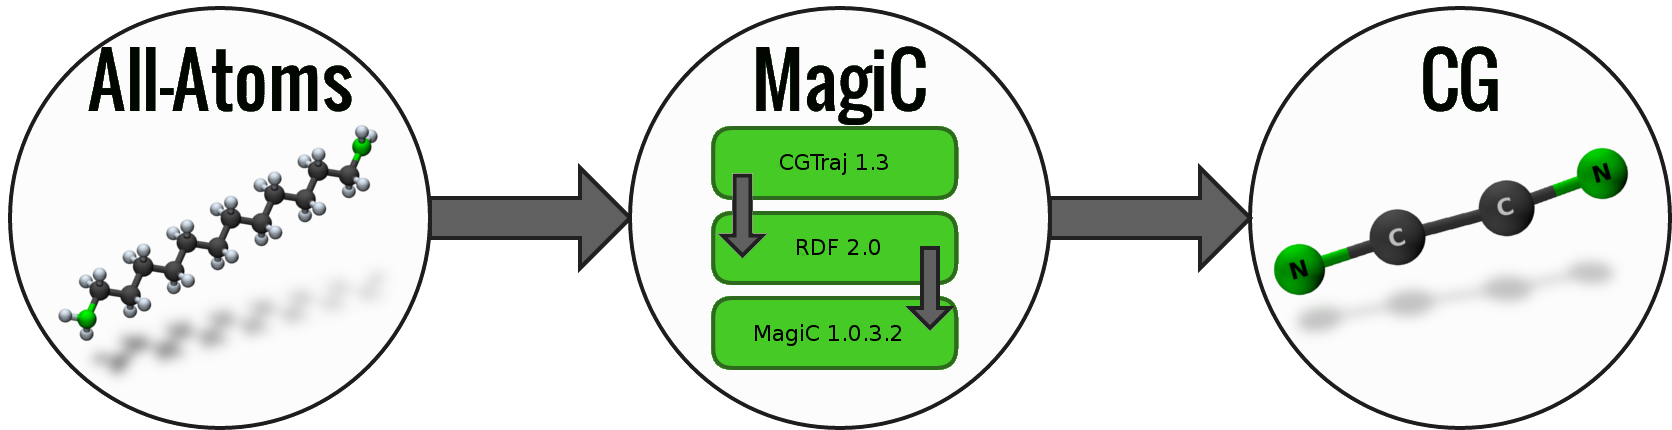
\includegraphics[width=1 \textwidth]{./images/magic}
	\caption{MagiC}
	\label{Fig:magic}
	\end{center}
	\end{figure}

 The first step uses "CGtraj 1.3" (MagiC package utility written in Fortran 90) \cite{magicmanu}, where the trajectory of the all-atoms simulation is recalculated based on a bead mapping described by the user. Basically, it analyses the group of atoms in each bead and assign the position of this bead as the center of mass, charge as summation of all charges and mass as summation of atomic masses, thus giving as output a representation of the input system as if it was an "ideal" coarse-grain model. Next, this rewritten trajectory is used as input to rdf-2.0  (MagiC package utility written in Python) \cite{magicmanu}, where several reference Radial Distributions Functions are created for each bond, angle and pairwise intermolecular interaction, as specified by user. These reference RDFs in conjunction with the coarse-grain topology are the  inputs to the MagiC kernel (MagiC package utility written in Fortran 90) \cite{magicmanu}, which is the key step of the process, where the final output might be a suitable coarse-grain model ready for GROMACS simulation.
 
 In the kernel is where the actual inversion precesses occurs, as schematised in Fig.(\ref{Fig:kernel}). Whether using IMC or IBI, a couple of millions of Metropolis Monte Carlo steps are simulated using a set of trial potentials to create several samples of averaged thermodynamics properties. Then, these averages are applied in the equations of the chosen inversion method in order to refine the trial potentials that will be used on the next inversion step.
 \begin{figure}[ht!]
  \begin{center}
	
\includegraphics[width=0.3 \textwidth]{./images/wip}
	\caption{MagiC kernel work-flow scheme}
	\label{Fig:kernel}
  \end{center}
\end{figure}
 
 The Iterative Boltzmann Inversion is a reasonable methodology to apply in the initials iterations, since it has fast convergence. The process derives from probability distribution function (Eq.(12)), thus for a pairwise particle interaction, the relationship between the reference RDF and Potential Mean Force (PMF) enables the use of an iterative method shown in Eq.(17) \cite{ibi}:
   \begin{equation}
\mathcal{U}^{(i+1)}(r) = \mathcal{U}^{(i)}(r) - \eta k_B T \ln{\left(\dfrac{\rho^{(i)}(r)}{\rho_{ref}(r)}\right)}
\label{eqn:ibi}
\end{equation}

 Where $\eta$ is a regulation parameter to avoid excessive variations. For a system in a canonical ensemble, temperature will be constant, hence the the potential is corrected for each iteration using the $\rho_{ref}(r)$ calculated from reference RDF in comparison to $\rho^{(i)}(r)$ from  RDF generated by Metropolis Monte Carlo simulation. Although this method is efficient to achieve small deviance from references, it does not guarantee that the generated potential represents one that will reproduce a behaviour similar to atomistic model because IBI does not consider cross-correlation terms between bonds and angles \cite{magic}.   
 
 Regarding the Inversion Monte Carlo process, it follows the methodology described by \citeA{imc}. Given a Hamiltonian, that means the total energy of the system:
 \begin{equation}
\mathcal{H}(q) = \displaystyle \int \mathcal{U}_\alpha\mathcal{S}_\alpha(q) \,d\alpha
\label{eqn:hami}
\end{equation}

For pair interactions, the degree of freedom $q$ in Eq.(\ref{eqn:hami}) becomes the distance $r$ between a pair of atoms. Therefore, for a real system the Hamiltonian would be the summation of an infinite set of $\mathcal{U}_\alpha$. However, a good approximation for numerical methods is to assume a cut-off radius $r_{\mathsf{cut}}$, where potentials no longer have relevant value after this point. One can define a $\Delta r = \dfrac{r_{\mathsf{cut}}}{\mathcal{M}}$, obtaining $\mathcal{M}$ subdivisions and thus a finite set of  $\mathcal{U}_{\alpha}$ in which $\mathcal{S}_\alpha$ is the number of pairs within  interval $[r_\alpha,(r_\alpha + \Delta r)]$. Since $\mathcal{S}_\alpha$ is function of $\mathcal{U}$, one can derive the following Taylor expansion:

 \begin{equation}
\Delta\left\langle\mathcal{S}_\alpha\right\rangle = \sum_{\phi=\alpha}^\mathcal{M}\dfrac{\partial\left\langle\mathcal{S}_\alpha\right\rangle}{\partial\mathcal{U}_\phi}\Delta\mathcal{U}_\phi + \mathcal{O}({\Delta\mathcal{U}_\phi}^2)
\label{eqn:inv1}
\end{equation}
 \begin{equation}
\dfrac{\partial\left\langle\mathcal{S}_\alpha\right\rangle}{\partial\mathcal{U}_\phi} = \dfrac{ \left\langle\mathcal{S}_\alpha\right\rangle\left\langle\mathcal{S}_\phi\right\rangle - \left\langle\mathcal{S}_\alpha\mathcal{S}_\phi\right\rangle}{k_B T}
\label{eqn:inv2}
\end{equation}

For each inversion step $k$, Monte Carlos simulations are run using a set of potentials $\mathcal{U}_{\alpha}^{(k)}$, then as explained previously it is possible to calculate ensemble averages of the cross-correlation terms ${\left\langle\mathcal{S}_\alpha\mathcal{S}_\phi\right\rangle}^{(k)}$ and averages $\left\langle\mathcal{S}_\alpha\right\rangle^{(k)}$, $\left\langle\mathcal{S}_\phi\right\rangle^{(k)}$. At this point, the reference RDFs becomes useful for inverse Monte Carlo. Since this method deals with pairwise interactions the value of $\mathcal{S}_\alpha$ and $\rho(r)$ are directly proportional following the rule $\mathcal{S}_\alpha^{*}= \rho(r_\alpha)\Delta r $ \cite{magic} because both measure the quantity of one type of coarse-grain bead in relation to another. Hence, by using $\Delta\left\langle\mathcal{S}_\alpha\right\rangle = \left\langle\mathcal{S}_\alpha\right\rangle^{(k)} - \mathcal{S}_\alpha^{*}$  in conjunction with Eq.(\ref{eqn:inv1}) and Eq.(\ref{eqn:inv2}) and neglecting the error $\mathcal{O}({\Delta\mathcal{U}}^2)$ the potential correction for next step $\Delta\mathcal{U}_\alpha^{(k)}$ can be obtained and finally potentials are updated using the following  equation:
 \begin{equation}
\mathcal{U}_\alpha^{(k+1)}= \mathcal{U}_\alpha^{(k)}+\Delta\mathcal{U}_\alpha^{(k)}
\label{eqn:inv2}
\end{equation} 

Both of the previous methods described rely on a considerably large mount of Monte Carlo simulation steps. That is due to the fact that the closer the set of potentials gets to solution the harder it becomes to distinguish between statistical noise and a suitable potential correction. For his reason, MagiC has a built-in capacity of running parallel Monte Carlo simulation as it an be see on Fig.(\ref{Fig:kernel}), which which enable the user to reach the order of billions of simulation steps in a feasible timespan. Moreover, there is not an unique solution for a given RDF \cite{ibi} and eventually solution can possible diverge at a certain point. Therefore, a satisfactory result depend on analysis of all outputs from inverse steps in order to guarantee convergence. Further explanations regrading functionalities and parameters for MagiC and GROMACS will be provided the next section.   
 
\subsection{Methods Description} 
\subsubsection*{GROMACS All-Atom simulations}
The experimental process of this project is divided in 3 main parts: Firstly, develop a efficient coarse-grain model and validate its use. Secondly, analyse the relationship between concentration  of all-atoms simulation and concentration of coarse-grained simulation. Then finally, create and reproduce a Silica surfactant mesoscale system. 

In order to maintain standard parameters for all GROMACS simulations, all-atoms simulations that were used for coarse-grained reference were run in NPT ensemble. All simulation boxes were created using genbox (GROMACS package utility), first by inserting the desired number of surfactant molecules and then adding the solvent at the adequate ratio. The molecules were designed based on OPLS-AA forcefield \cite{opls} parameters. %because?%
The surfactant DMDD was created with aid of co-workers and water type was TIP4P \cite{tip4p}. %because?% 
Moreover, no initial configuration was determined, such as a pre self-assembled system, to ensure stochastic nature of the system.  

Initially, all boxes received a energy minimization step in order to avoid system blow-up deal to possible extreme potential energy spots created during box generation. That is because during random displacement of molecules some of them could overlap others and then cause a destabilization of the system. After, an equilibration step was necessary to reach desired initial temperature and pressure conditions for the MD simulation. During equilibration temperature coupling was kept at $298\ K$ using a v-rescaling thermostat \cite{vtstat} with time constant of $0.01\ ps$ and pressure coupling was kept at $1\ bar$ using a Berendsen barostat \cite{bbtat} with time constant of $0.5\ ps$.  The simulation was run for $200\ ps$ with time step of $0.5\ fs$ using leap-frog algorithm.

Regarding the concentration of surfactant in each box, four all-atom boxes were created with composition and size described in Table (\ref{tab:boxes}). 
\begin{table*}[ht!] 
  \centering
\begin{threeparttable}

  \caption{Description of all-atom simulation boxes}

    \begin{tabular}{cccccc}
    \toprule
    Box &  DMDD &  Water & Silica & Avg. size & Concentration \\
	& (no. Molec.) & (no. Molec.) & (no. Molec.)  & (\AA) & (mM)\\
    \midrule
    1   & 30  & 1500  & -  & 38.2646 & 0.89\\
    2   & 30  & 670  & -   &  31.3201 & 1.62\\
    3   & 45\tnote{a}  & 240  & -  & 28.2972 & 3.30\\
    4   & 30  & 670  &  30  & ??? & ???\\
    \bottomrule
    \end{tabular}%
    \begin{tablenotes}
    	\item[a] Necessary change, otherwise box size would be too small for the experiments, however concentration is the same as a 30-160 box.
    \end{tablenotes}
  \label{tab:boxes}%
\end{threeparttable} 
\end{table*}

The utility of each box will be described further in each experiment section. Even though they have different structural parameters, all of them followed the same ensemble with temperature kept at $298\ K$ by a Nosé-Hoover thermostat \cite{nosetstat} and pressure kept at $1\ bar$ by a Parrinello-Rahman barostat \cite{prbstat}. Moreover, simulation time was also standardized. Every simulation lasted $350\ ns$ with a time step of $0.1\ fs$ using leap-frog algorithm. But for the sake of experiments using MagiC, the first $50\ ns$ of the simulations were disregarded because during this time the system still in equilibration, and therefore that would affect reference RDF values.


\subsubsection*{Experiment 1}
 Since the main objective of this project is to probe the effectiveness of coarse-grain models generated using MagiC, this first experiment is an attempt to understand and analyse to what extent bead size influence on the process of coarse-graining. Hence, two models were proposed: Model 1 (M1) described in Fig.(\ref{Fig:mol1}) and Model 2 (M2) described in Fig. (\ref{Fig:mol2}).
 
 \begin{figure}[ht]
	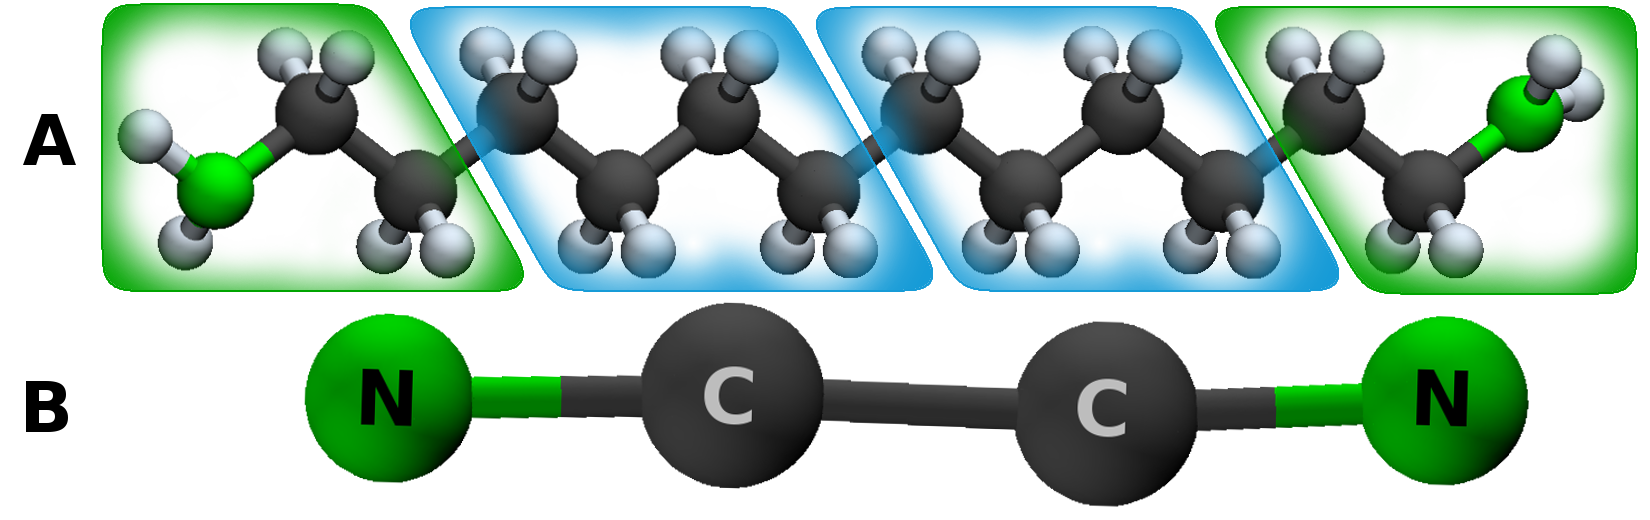
\includegraphics[width=1.0 \textwidth]{./images/M1ab}
	\caption{A) Schematic of M1 molecule split plan, Carbon atoms represented in black, Nitrogen in green and Hydrogen in gray. B)Final coarse-grain model for M1. This model aggregated the three most polar heavy atoms on the tips and four apolar heavy atoms at the center.}
	\label{Fig:mol1}
\end{figure}
 \begin{figure}[ht]
	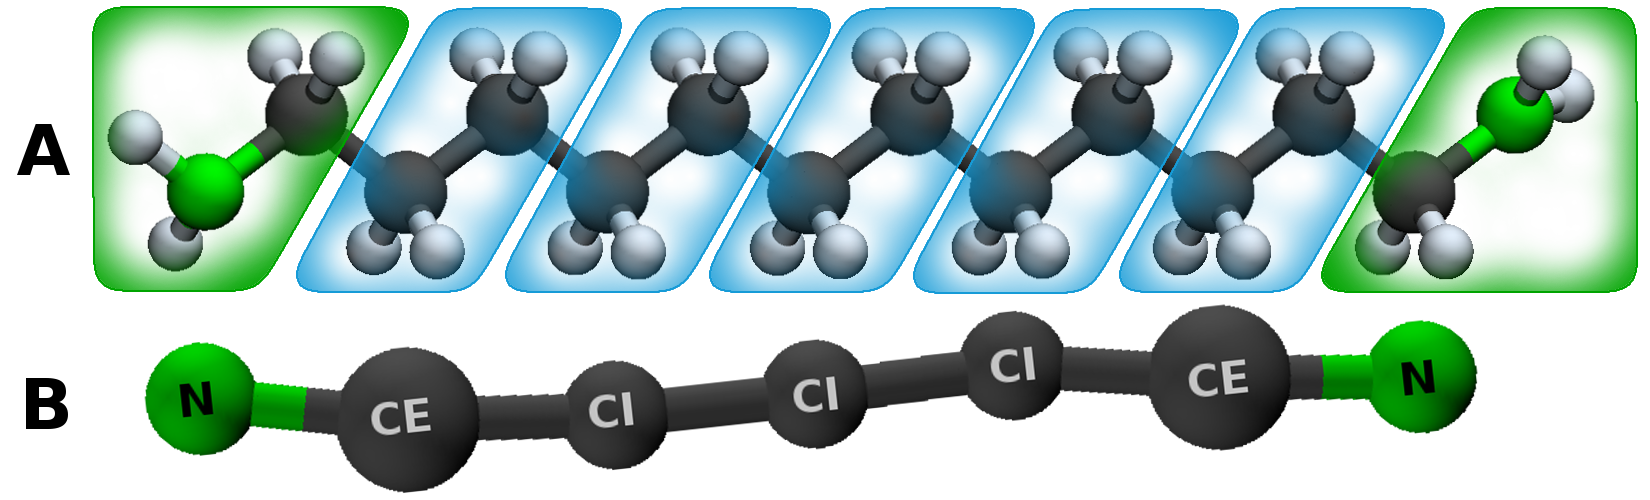
\includegraphics[width=1.0 \textwidth]{./images/M2ab}
	\caption{A) Schematic of M2 molecule split plan, Carbon atoms represented in black, Nitrogen in green and Hydrogen in gray. B)Final coarse-grain model for M2. Heavy atom were grouped pairwise in such a manner that amphiphilic parts were kept as distinct as possible. It is important to notice the necessity of two carbon bead types CE and CI}
		\label{Fig:mol2}
\end{figure}
 
 The differences between M1 and M2 are an effort to distinguish at different level of detail the amphiphilic nature of the DMDD. In order to avoid electrostatic interactions on the IMC process and further GROMACS simulations, the heavy atom groups (heavy atom + hydrogen) were kept together, thus  final charge remain neutral in each bead. Hence, forces will only arise from Van der Waals interactions and implications of inverse process might originate from  degrees of freedom deal to number of beads.
 
 In order to fully describe the system, MagiC will generate potential tables for interaction between each bead. The first type of table are for each bound type, for example on M1, there are two different tables: one for N-C bond and other for C-C bond. However, as soon as the molecule is symmetric the two external N-C bonds uses the same potential table. Secondly, it generates tables for each angle type, following the symmetry rule. And finally, each type interatomic pair interaction has its own table, i.e. on M1 there are three: N-N, N-C and C-C. A more detailed description for both models is exposed in Table (\ref{tab:potdes}).
  
 \begin{table*}[ht!] 
  \centering
\begin{threeparttable}

  \caption{Description of coarse-grain models}

    \begin{tabular}{c|c|c|c}
    \toprule
    &  Bonds & Angles & Interatomic \\
    \midrule
    Model 1   & [N-C] [C-C]  & [N-$\widehat{C}$-C]  & [N-N] [N-C] [C-C]  \\
    \midrule
      			& [N-CE]  & [N-$\widehat{CE}$-CI]  & [N-N] [N-CE]   \\
      Model 2	& [CE-CI] &  [CE-$\widehat{CI}$-CI] &  [N-CI] [CE-CE]   \\
     			 & [CI-CI]  &  [CI-$\widehat{CI}$-CI] &  [CE-CI] [CI-CI]  \\
    \bottomrule
    \end{tabular}%
  \label{tab:potdes}%
\end{threeparttable} 
\end{table*}

 When using MagiC package the model description begins at the "CGtraj" step, where the user need to describe what are the bead types for the model and which atoms will be inside each bead. These informations must be part of input file of "CGtraj", following the strict guidelines of MagiC Manual \cite{magicmanu}. At the second step is where bonds, angles, and interatomic interactions must be described in the input file for "rdf-2.0" utility, following as well MagiC Manual guidelines \cite{magicmanu}.  That is because at this point MagiC will generate reference RDF's used in inversion process for each potential table. Additional information regarding model description in input files for M1 and M2 can be found on Appendix (see Section \ref{sec:appendix}).
 
 --IMC process\\
 --gromacs Set-up Reproduction Tests
\subsubsection*{Experiment 2}
 --Objective\\
 --gromacs Set-up Up-scaling \\
 --gromacs Set-up Self-assembly Model X(best)\\
  ----AA Low, CG Low\\
   \begin{figure}[ht!]
  \begin{center}
	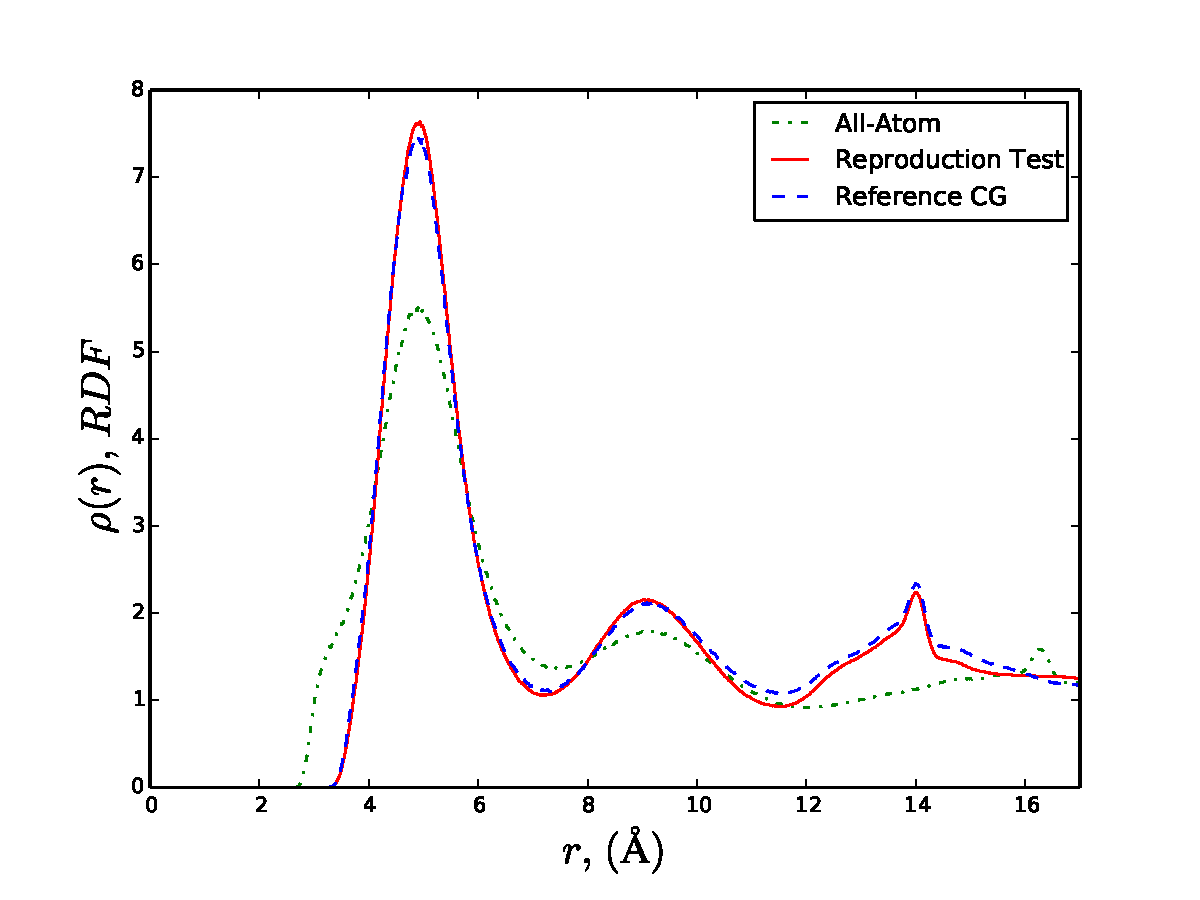
\includegraphics[width=1 \textwidth]{./graphs/rdfL}
	\caption{rdfLow}
		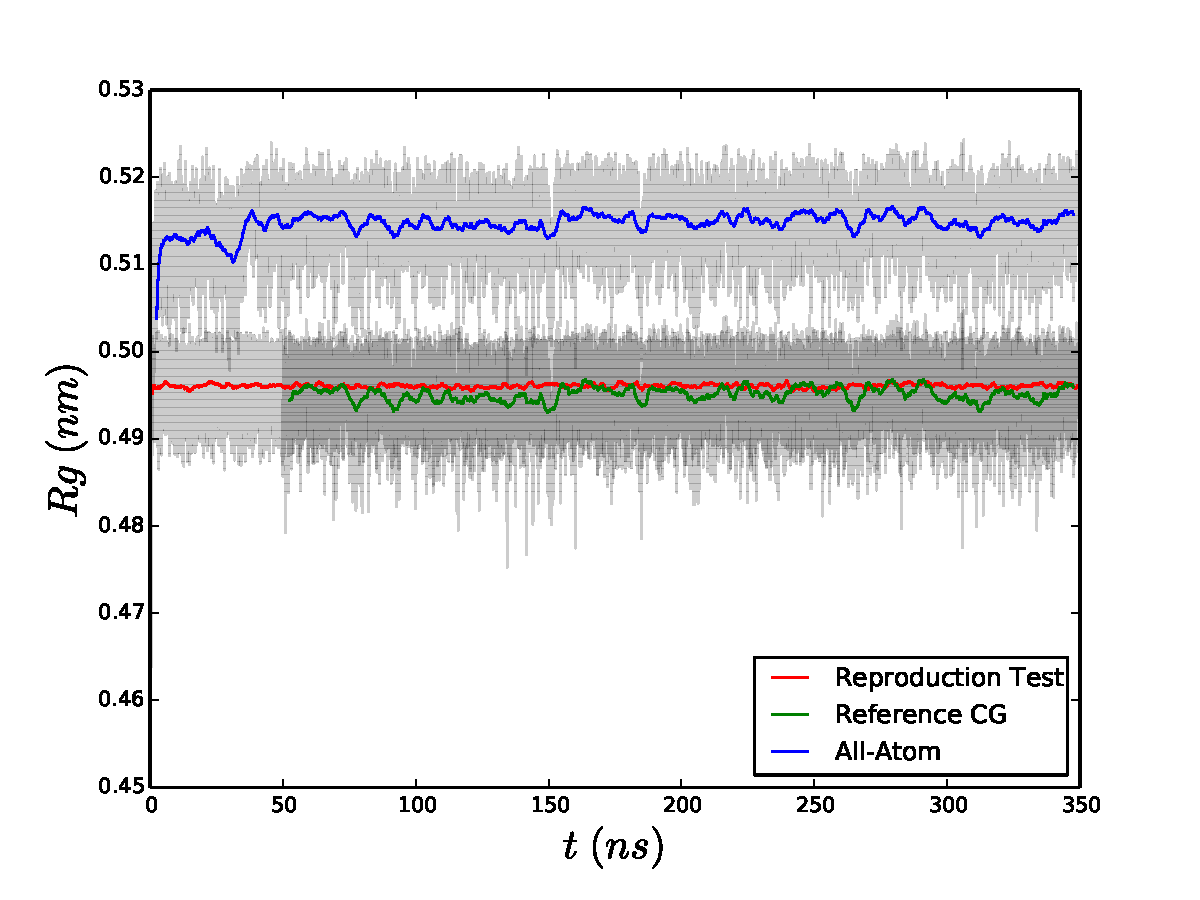
\includegraphics[width=1 \textwidth]{./graphs/GyraL}
	\caption{Gyration Low}
	\label{gfx:rdfLow}
	\end{center}
	\end{figure}
   ------1k(?) up-scale @ low\\
   ------1k(?) up-scale @ high\\
  ----AA Ideal, CG ideal\\
     \begin{figure}[ht!]
  \begin{center}
	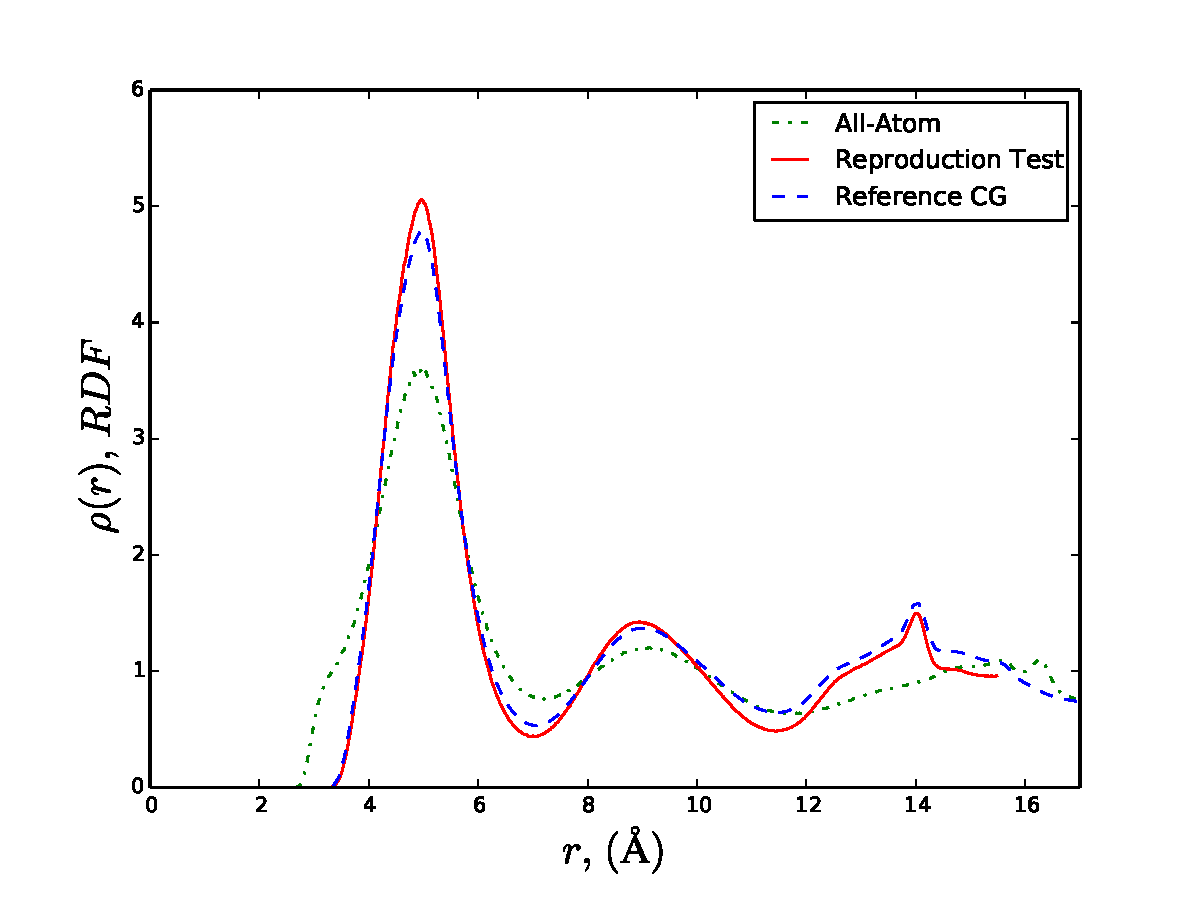
\includegraphics[width=1 \textwidth]{./graphs/rdfI}
	\caption{rdfIdeal}
		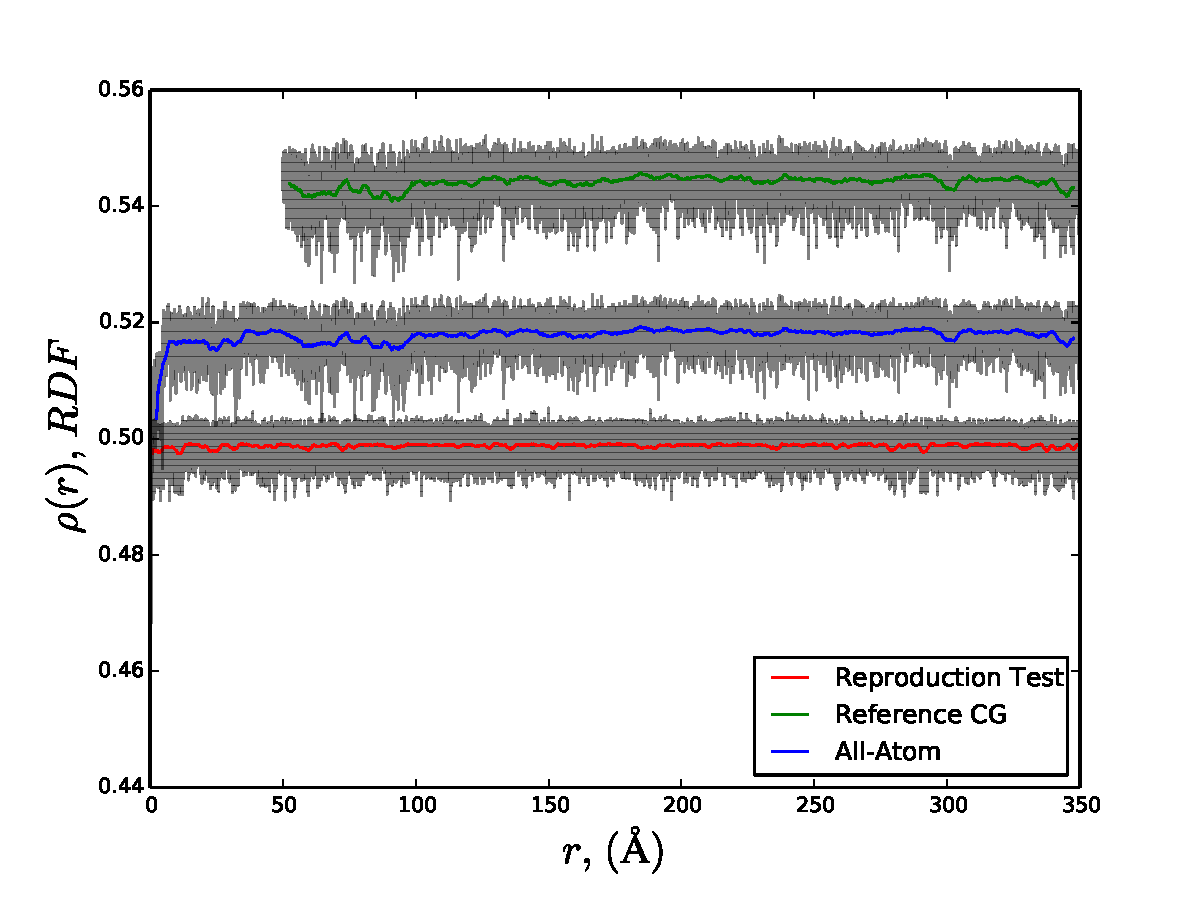
\includegraphics[width=1 \textwidth]{./graphs/GyraI}
	\caption{Gyration Ideal}
	\label{gfx:rdfI}
	\end{center}
	\end{figure}
   ------1k(?) up-scale @ low\\
   ------1k(?) up-scale @ ideal\\
   ------1k(?) up-scale @ high  \\
  ----AA High, CG High\\
   ------1k(?) up-scale @ high\\
   ------1k(?) up-scale @ high
\subsubsection*{Experiment 3}
 --Silica addition\\
  ----MagiC CG silica topology \\
  ----gromacs Set-up Self-assembly Model X + Si\\
   ------1000, 10000 (Maybe more?)
 
\section{Results}

Experiment 1\\
 --Model 1 vs Model 2 \\
 --gromacs Simulation\\
 --IMC process Convergence\\
 --gromacs Reproduction Tests RDFs and Properties\\
Experiment 2\\
 --Self-assembly vs concentration Model X\\
  ----Ideal con validation: Low, Ideal, High con comparison\\
   ------Ideal @ Low -> validate\\
   ------Ideal @ Ideal -> evaluate\\
   ------Ideal @ High -> validate\\
  ----Extremes evaluation:\\
  ------Low @ Low vs High @ Low -> compare\\
   ------High @ High vs Low @ High -> compare\\
Experiment 3\\
 --Silica addition\\
  --CG silica Properties \\
  --Self-assembly Model X + Si\\
   -----1000, 10000 (Maybe more?)\\

\section{Discussion}

%The purpose of the discussion is to interpret and compare the results. Be objec
%tive; point out the features and limitations of the work. Relate your results to cur
%rent knowledge in the field and to the original purpose in undertaking the project:
%Was the problem resolved? What has been contributed? Briefly state the logical
%implications of the results. Suggest further study or applications if warranted.

Experiment 1\\
 --Which is the best Model?\\
 --Why Model X is better than Model Y?\\
 --To what extent Model X represent well the AA model?\\
 --What are the limitations and advantages of Model X?\\
Experiment 2\\
 --What is the relation between the entropy "error" and concentration? \\
 --Is the concentration really an problem?\\
 --Do you need to run an AA for each con or the Ideal can represent any?\\
 --Even extreme cases can be approximated? In this case how much is the "error"?\\
Experiment 3\\
 --Is The silica CG model suitable? \\
 --Can you the proprieties validate it?\\
 --The self-assembly behaviour change with silica addition?\\

\section{Conclusion}

 %Make a fair conclusion... Repeating the results is not drawing a conclusion...
 What did you really see from the results?\\
 There was any bad assumption that is contestable?\\
 What will be the next step to your research? \\
 
\section{Nomenclature} 
   \begin{tabulary}{1.0\textwidth}{LCL}
   $\mathcal{H}$ &   & Hamiltonian \\
   $k_B$ & & Boltzmann's Constant\\
   $C_n$ &   & Molar concentration of species n ($mM$) \\
   \end{tabulary}

\bibliography{./biblio/biblio}
\vfill
\newpage
\section{Appendix}
\label{sec:appendix}
\setcounter{page}{1}
\begin{equation}
E_c=\frac{1}{2}mv^2
\label{eqn:bua}
\end{equation}

\begin{table*}[ht!] 
  \centering
\begin{threeparttable}

  \caption{Table generated by Excel2LaTeX from sheet 'Sheet1'}

    \begin{tabular}{rrrrrr}
    \toprule
    Model & Depth & Width & Angle & Factor 1 & Factor 2 \\
	& (mm) & (mm) & (°)  &  &  \\
    \midrule
    111   & 1,00  & 1,50  & 10\tnote{a}   & 357.921 & 532.289 \\
    112   & 1,00  & 1,50  & 15   & 382.379 & 567.234 \\
    113   & 1,00  & 1,50  & 20   & 383.863 & 569.600 \\
    121   & 1,00  & 2,00  & 10   & 398.199 & 590.473 \\
    122   & 1,00  & 2,00  & 15   & 486.306 & 710.483 \\
    123   & 1,00  & 2,00  & 20   & 430.330 & 636.471 \\
    131   & 1,00  & 2,50  & 10   & 441.735 & 654.499 \\
    132   & 1,00  & 2,50  & 15   & 460.925 & 681.645 \\
    133   & 1,00  & 2,50  & 20   & 469.115 & 693.700 \\
    211   & 1,25  & 1,50  & 10   & 374.784 & 557.029 \\
    212   & 1,25  & 1,50  & 15   & 399.053\tnote{b} & 591.402 \\
    213   & 1,25  & 1,50  & 20   & 411.377 & 609.042 \\
    221   & 1,25  & 2,00  & 10   & 415.050 & 615.336 \\
    222   & 1,25  & 2,00  & 15   & 430.991 & 638.237 \\
    223   & 1,25  & 2,00  & 20   & 455.857 & 673.613 \\
    231   & 1,25  & 2,50  & 10   & 472.885 & 698.958 \\
    232   & 1,25  & 2,50  & 15   & 484.567 & 715.341 \\
    233   & 1,25  & 2,50  & 20  & 497.320 & 733.923 \\
    311   & 1,50  & 1,50  & 10   & 385.110 & 572.665 \\
    312   & 1,50  & 1,50  & 15   & 406.144 & 602.130 \\
    313   & 1,50  & 1,50  & 20   & 480.613 & 706.960 \\
    321   & 1,50  & 2,00  & 10   & 490.910 & 722.194 \\
    322   & 1,50  & 2,00  & 15   & 513.846 & 754.804 \\
    323   & 1,50  & 2,00  & 20   & 529.291 & 777.175 \\
    331   & 1,50  & 2,50  & 10   & 542.184 & 796.618 \\
    332   & 1,50  & 2,50  & 15   & 510.958 & 753.298 \\
    333   & 1,50  & 2,50  & 20   & 527.253 & 776.981 \\
         \midrule
          &       &       & Sum: & 12.138.966 & 17.932.100 \\
    \bottomrule
    \end{tabular}%
    \begin{tablenotes}
    	\item[a] This should be cited with a \citeA{magic}
    	\item[b] And this is another note
    \end{tablenotes}
  \label{tab:addlabel}%
\end{threeparttable} 
\end{table*}

\begin{figure}[ht!]
  \begin{center}
	
\includegraphics[width=0.3 \textwidth]{./images/wip}
	\caption{Work in Progress}
	\label{Fig:Boxplot}
  \end{center}
\end{figure}

\end{document}